\documentclass[journal,12pt,twocolumn]{IEEEtran}
\usepackage{graphicx}
\graphicspath{{./figs/}}{}
\usepackage{amsmath,amssymb,amsfonts,amsthm}
\newcommand{\myvec}[1]{\ensuremath{\begin{pmatrix}#1\end{pmatrix}}}
\usepackage{listings}
\usepackage{watermark}
\usepackage{titlesec}
\let\vec\mathbf

\titlespacing{\subsection}{0pt}{\parskip}{-3pt}
\titlespacing{\subsubsection}{0pt}{\parskip}{-\parskip}
\titlespacing{\paragraph}{0pt}{\parskip}{\parskip}
\newcommand{\figuremacro}[5]{
    
}
\lstset{
frame=single, 
breaklines=true,
columns=fullflexible
}
\thiswatermark{\centering \put(0,-105.0){
\includegraphics[scale=0.08]{logo.jpg}} }

\sloppy
\title{\mytitle}
\title{
Optimisation
}
\author{T.Sai Raghavendra}
\begin{document}
\maketitle
\tableofcontents
\bigskip


\section{\textbf{Problem Statement}}
Let f(x) = $sin^3 x+\lambda sin^2 x, \frac{-\pi}{2} < x < \frac{\pi}{2} $. Find the intervals in which $\lambda$ should lie in order that f(x) has exactly one minimum and exactly one maximum.\\


\section{\textbf{Solution}}
Given function is ,
	\begin{align}
	\label{eq:one}
	f(x)= sin^3 x+\lambda sin^2 x
	\end{align}
	$\vec{Theoritical proof:}$\\ \\
Let y=f(x)=$sin^3 x+\lambda sin^2 x, \frac{-\pi}{2} < x < \frac{\pi}{2} $\\ \\
Let $sinx=t$
    \begin{align}
	 \frac{dy}{dt}=3t^2+2t\lambda=t(3t+2\lambda)
	 \end{align}
	 for exactly one minima and exactly one maxima  $\frac{dy}{dx} $ must have two distinct roots $\in$ (-1,1) \\
	 $t=0$ and $t=\frac{-2\lambda}{3}\in (-1,1)$\\
	 \begin{align}
	 -1<\frac{-2\lambda}{3}<1\\
	 \frac{-3}{2}<\lambda<\frac{3}{2}\\
	 \lambda\in (\frac{-3}{2},\frac{3}{2})
	 \end{align}
	$\vec{Objective function:}$
	\begin{align}
	\min_xf(x)= sin^3 x+\lambda sin^2 x, \frac{-\pi}{2} < x < \frac{\pi}{2} \\
	\max_xf(x)= sin^3 x+\lambda sin^2 x, \frac{-\pi}{2} < x < \frac{\pi}{2} 
        \end{align}
	$\vec{constraints:}$
	\begin{align}
		x \in \{ \frac{-\pi}{2}, \frac{\pi}{2}\} 
	\end{align}
\small$\vec{Calculation of Minima using gradient descent algorithm:}$
{Minima of the above \eqref{eq:one}, can be calculated from the following expression,}
Differentiating \eqref{eq:ten} yields,
\begin{align}
       \boxed{x_{n+1} = x_n - \alpha \nabla h(x_n)}\\
       \label{eq:ten}
		f(x)= sin^3 x+\lambda sin^2 x \\ 
		\nabla f(x) = sinx cosx (3sinx+2\lambda) 
\end{align}
Taking $x_0=\frac{-\pi}{2},\alpha=0.0001$ and precision = 0.000000001, values obtained using python are:
    \begin{align}
        \boxed{\text{Minima} =-2.5}\\     
        \boxed{\text{Minima Point} = -1.5708}
    \end{align}
   
\small$\vec{Calculation of Maxima using gradient ascent algorithm:}$
{Maxima of the above \eqref{eq:one}, can be calculated from the following expression,}
Differentiating \eqref{eq:fifteen} yields,
\begin{align}
       \boxed{x_{n+1} = x_n - \alpha \nabla h(x_n)}\\
       \label{eq:fifteen}
	f(x)= sin^3 x+\lambda sin^2 x \\ 
	\nabla f(x) = sinx cosx (3sinx+2\lambda)
\end{align}
Taking $x_0=\frac{\pi}{2},\alpha=0.0001$ and precision = 0.000000001, values obtained using python are:
    \begin{align}
        \boxed{\text{Maxima} =2.5}\\     
        \boxed{\text{Maxima Point} = 1.5707}
    \end{align}
\section{\textbf{Plots}}
\begin{figure}
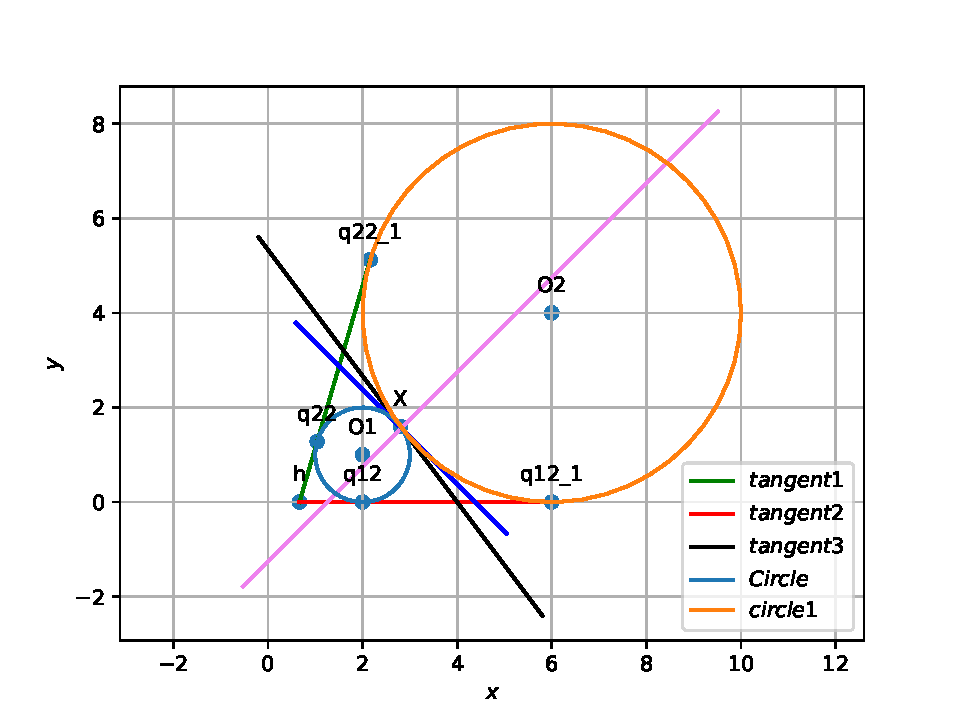
\includegraphics[width=\columnwidth]{fig.pdf}
\caption{Minima of $\lambda \in \{\frac{-3}{2},\frac{3}{2}\}$}
\label{fig:Figure}
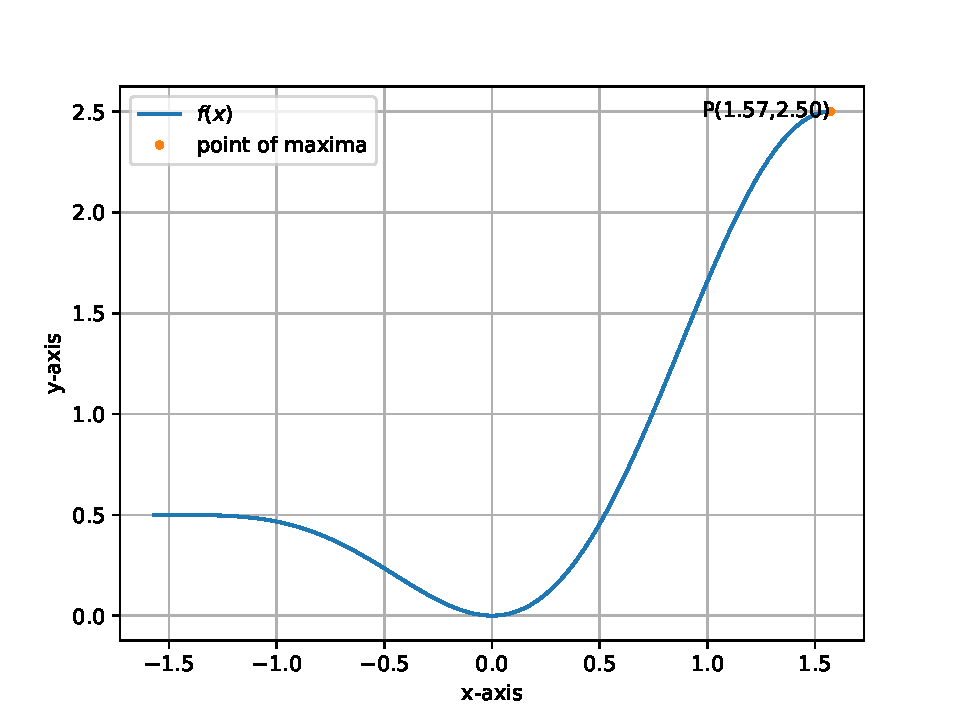
\includegraphics[width=\columnwidth]{fig1.pdf}
\caption{Maxima of $\lambda \in \{\frac{-3}{2},\frac{3}{2}\}$}
\label{fig:Figure}
\end{figure}
Violation of $\lambda$:\\ 
$\lambda$ violate the given condition beyond this range 
\begin{center}
$x \in \{ \frac{-3}{2}, \frac{3}{2}\}$
\end{center}
 
Let us consider $\lambda$ beyond this range  \\
considering, $\lambda \in \{-5,-2\}$ and
\begin{figure}
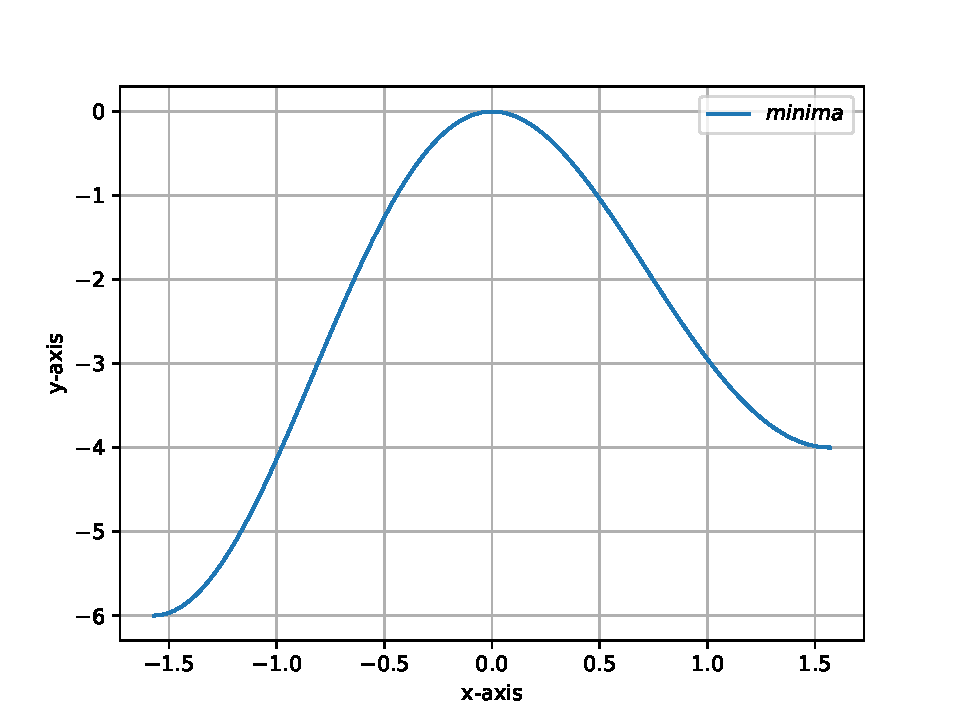
\includegraphics[width=\columnwidth]{fig3.pdf}
\caption{Minima of $\lambda \in \{-5,-2\}$}
\label{fig:Figure}
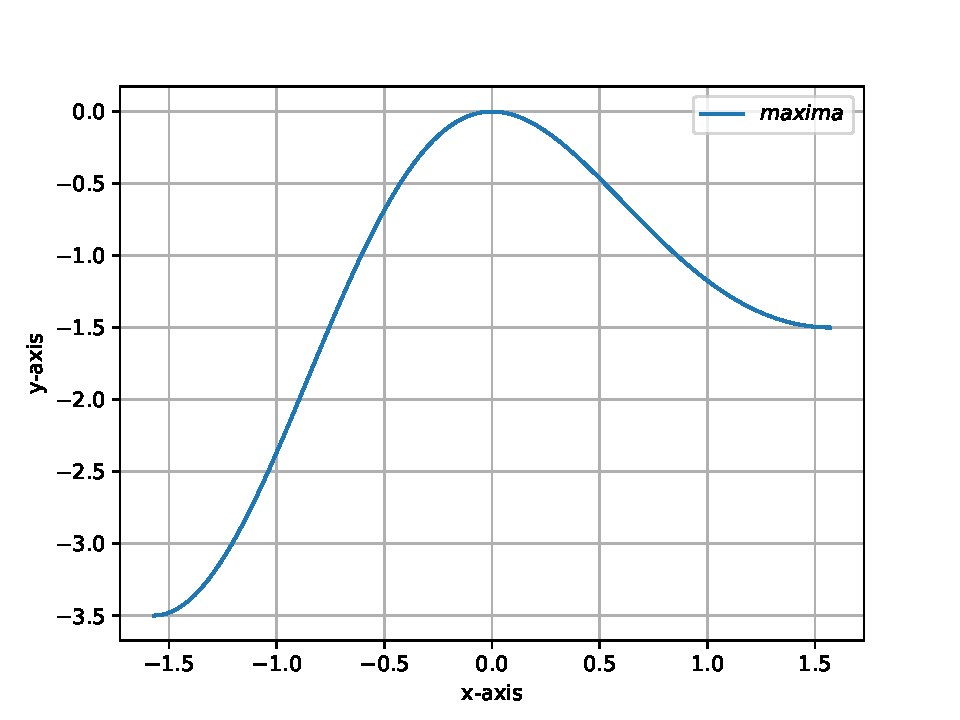
\includegraphics[width=\columnwidth]{fig4.pdf}
\caption{Maxima of $\lambda \in \{-5,-2\}$}
\label{fig:Figure}
\end{figure}
$\lambda \in \{2,5\}$
\begin{figure}
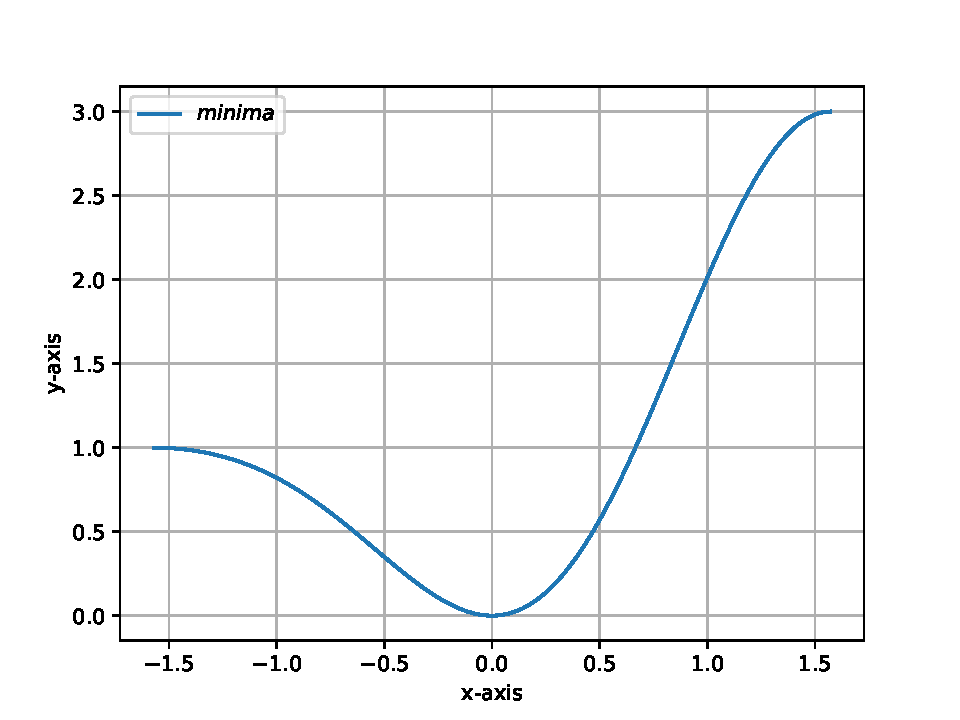
\includegraphics[width=\columnwidth]{fig5.pdf}
\caption{Minima of $\lambda \in \{2,5\}$}
\label{fig:Figure}
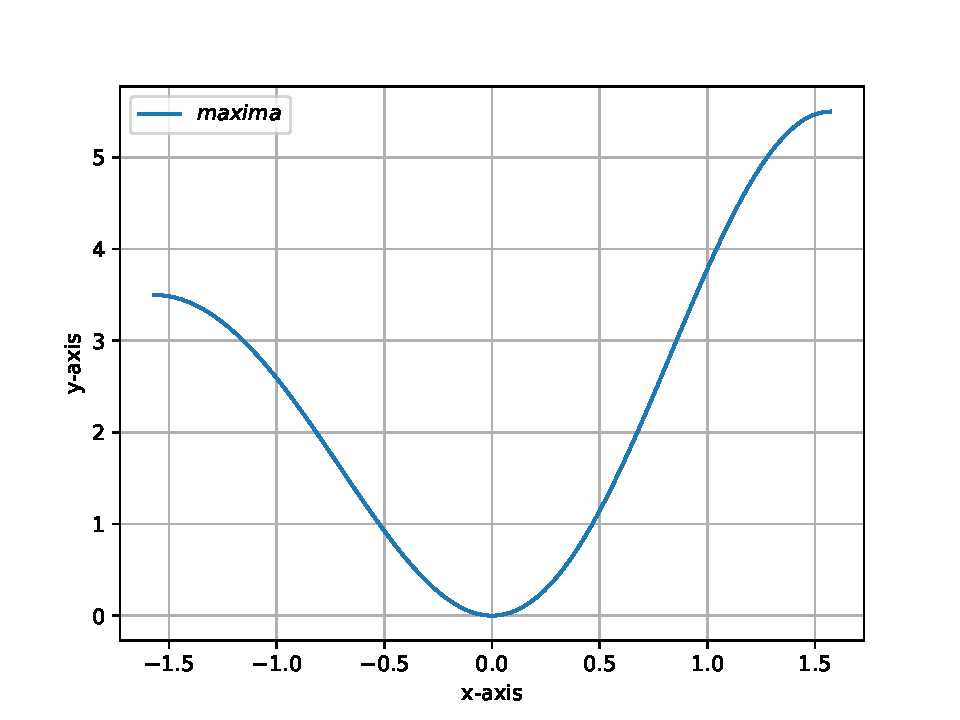
\includegraphics[width=\columnwidth]{fig6.pdf}
\caption{Maxima of $\lambda \in \{2,5\}$}
\label{fig:Figure}
\end{figure}

\section{\textbf{Software}}
\begin{lstlisting}
https://github.com/Sairaghavendra36/Fwc-2022/blob/main/Matrix/Optimisation/opti.py
\end{lstlisting}

\end{document}





